% =====================================================================
\section{The Objects, Part by Part}\label{sec:construction}
\pipestrip{2}
A composite object is a small scene graph: leaves draw one primitive with their own $S,R,T$; group nodes carry a transform and a name. Table~\ref{tab:parts} is
generated from the export: the scene holds \nLeaves{} leaf parts in \nObjects{} objects. T38 checks that every
leaf is a cube, sphere, cylinder or cone; T70/T67/T96/T99 check each object for ``primitives only, every node named''.

\begin{table}[h]
\centering\small
\caption{Parts per composite object, generated from \code{build/scene\_export.json}. Depth is the deepest group
level. The \emph{Target Rover} row counts all three intruders (\partsRover{} parts each). }
\label{tab:parts}
% generated by report/gen_tables.py from build/scene_export.json -- do not edit
\begin{tabular}{@{}lrrrp{4.6cm}l@{}}
\toprule
Object (export name) & Parts & Groups & Depth & Cube / Sphere / Cylinder / Cone / Frustum & Shading\\\midrule
Terrain & 1 & 1 & 1 & 1 height-field disc & Gouraud 1\\
Backdrop & 120 & 47 & 3 & 0 / 24 / 10 / 86 / 0 & Gouraud 120\\
Environment & 652 & 89 & 3 & 46 / 201 / 237 / 168 / 0 & Gouraud 652\\
Command Bunker & 400 & 17 & 3 & 291 / 19 / 90 / 0 / 0 & Flat 400\\
Autonomous UAV & 158 & 34 & 3 & 68 / 26 / 54 / 8 / 2 & Phong 156,\allowbreak{} Additive beam 2\\
Base & 1253 & 33 & 3 & 558 / 41 / 654 / 0 / 0 & Flat 616,\allowbreak{} Gouraud 637\\
Target Rover & 156 & 12 & 2 & 36 / 72 / 48 / 0 / 0 & Phong 156\\
Main Battle Tank & 255 & 29 & 5 & 170 / 5 / 80 / 0 / 0 & Phong 255\\
Scout Helicopter & 91 & 19 & 7 & 40 / 21 / 28 / 1 / 1 & Phong 90,\allowbreak{} Additive beam 1\\
AA Gatling Gun & 78 & 5 & 4 & 19 / 5 / 54 / 0 / 0 & Phong 78\\
Air-defence radar & 108 & 4 & 4 & 62 / 3 / 42 / 1 / 0 & Phong 108\\
SAM launcher & 112 & 9 & 4 & 74 / 5 / 32 / 1 / 0 & Phong 112\\
MLRS rocket truck & 136 & 22 & 4 & 45 / 9 / 76 / 6 / 0 & Phong 136\\
Main Battle Tank 2 & 255 & 29 & 5 & 170 / 5 / 80 / 0 / 0 & Phong 255\\
Main Battle Tank 3 & 255 & 29 & 5 & 170 / 5 / 80 / 0 / 0 & Phong 255\\
Ammunition bunker & 43 & 2 & 2 & 19 / 10 / 14 / 0 / 0 & Gouraud 43\\
Camp camouflage & 658 & 21 & 2 & 277 / 48 / 309 / 24 / 0 & Gouraud 658\\
Boom barrier & 20 & 2 & 2 & 17 / 2 / 1 / 0 / 0 & Gouraud 20\\
Windsock & 15 & 7 & 7 & 1 / 0 / 14 / 0 / 0 & Gouraud 15\\
Flag & 47 & 14 & 14 & 40 / 2 / 5 / 0 / 0 & Gouraud 47\\
Soldier 1 & 75 & 20 & 7 & 16 / 39 / 20 / 0 / 0 & Phong 75\\
Soldier 2 & 75 & 20 & 7 & 16 / 39 / 20 / 0 / 0 & Phong 75\\
Soldier 3 & 75 & 20 & 7 & 16 / 39 / 20 / 0 / 0 & Phong 75\\
Soldier 4 & 75 & 20 & 7 & 16 / 39 / 20 / 0 / 0 & Phong 75\\
Soldier 5 & 75 & 20 & 7 & 16 / 39 / 20 / 0 / 0 & Phong 75\\
Soldier 6 & 75 & 20 & 7 & 16 / 39 / 20 / 0 / 0 & Phong 75\\
Soldier 7 & 75 & 20 & 7 & 16 / 39 / 20 / 0 / 0 & Phong 75\\
Soldier 8 & 75 & 20 & 7 & 16 / 39 / 20 / 0 / 0 & Phong 75\\
Sky Clock & 1 & 1 & 1 & 0 / 1 / 0 / 0 / 0 & Gouraud 1\\
\midrule
Total & 5414 & 586 & & &\\
\bottomrule
\end{tabular}

\end{table}

\noindent The hierarchy diagrams are generated from the export: \emph{[n]} is the number of leaf
parts below a node, ``$\times k$'' collapses $k$ identical sibling groups, and italic lines summarise leaves directly under a group.

% ---------------------------------------------------------------------
\begin{figure}[h]
\centering
\picsheet{sheet_hierarchy}{\linewidth}
\caption{\sheetcaption{sheet_hierarchy}}
\end{figure}
\subsection{Underground command bunker}
\sheetfig{s03_primitive_mix}
\sheetfig{s03_bunker}
The bunker (\partsBunker{} parts, Flat shading) is underground: an entrance trench follows the vehicle track down a 7\,m ramp
($z=13\to6$) to the blast-door plane at $z=4$; behind it a tunnel leads to the command centre (CIC), a bunk room, a generator room and an emergency shaft with a ladder to a surface
hatch. All rooms share the floor level $y=-3.4$\,m; the terrain stays at least 0.15\,m above the roof slab (T60). Consoles in the CIC use the procedural \emph{Screen} surface. The two door leaves and two beacon spinners are animated (Section~\ref{sec:control}).

\begin{figure}[h]
\centering
\begin{minipage}[t]{0.52\linewidth}\vspace{0pt}% generated by report/gen_tables.py from build/scene_export.json -- do not edit
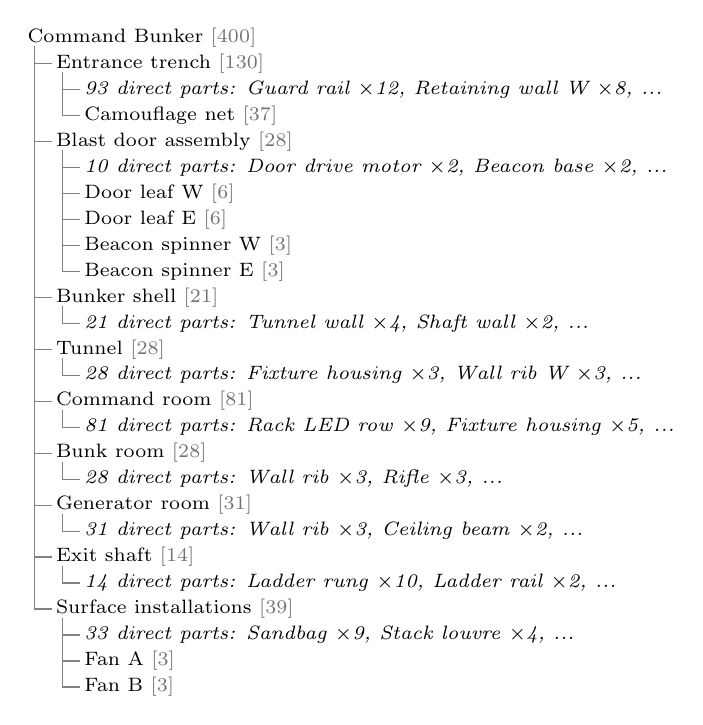
\begin{tikzpicture}[x=0.36cm,y=-0.33cm,font=\scriptsize]
\node[anchor=west,inner sep=0pt] (n0) at (0,0) {Command Bunker \textcolor{black!55}{[400]}};
\node[anchor=west,inner sep=0pt] (n1) at (1,1) {Entrance trench \textcolor{black!55}{[130]}};
\draw[black!50,thin] (0.25,0.35) |- (0.88,1);
\node[anchor=west,inner sep=0pt] (n2) at (2,2) {\textit{93 direct parts: Guard rail $\times$12, Retaining wall W $\times$8, ...}};
\draw[black!50,thin] (1.25,1.35) |- (1.88,2);
\node[anchor=west,inner sep=0pt] (n3) at (2,3) {Camouflage net \textcolor{black!55}{[37]}};
\draw[black!50,thin] (1.25,1.35) |- (1.88,3);
\node[anchor=west,inner sep=0pt] (n4) at (1,4) {Blast door assembly \textcolor{black!55}{[28]}};
\draw[black!50,thin] (0.25,0.35) |- (0.88,4);
\node[anchor=west,inner sep=0pt] (n5) at (2,5) {\textit{10 direct parts: Door drive motor $\times$2, Beacon base $\times$2, ...}};
\draw[black!50,thin] (1.25,4.35) |- (1.88,5);
\node[anchor=west,inner sep=0pt] (n6) at (2,6) {Door leaf W \textcolor{black!55}{[6]}};
\draw[black!50,thin] (1.25,4.35) |- (1.88,6);
\node[anchor=west,inner sep=0pt] (n7) at (2,7) {Door leaf E \textcolor{black!55}{[6]}};
\draw[black!50,thin] (1.25,4.35) |- (1.88,7);
\node[anchor=west,inner sep=0pt] (n8) at (2,8) {Beacon spinner W \textcolor{black!55}{[3]}};
\draw[black!50,thin] (1.25,4.35) |- (1.88,8);
\node[anchor=west,inner sep=0pt] (n9) at (2,9) {Beacon spinner E \textcolor{black!55}{[3]}};
\draw[black!50,thin] (1.25,4.35) |- (1.88,9);
\node[anchor=west,inner sep=0pt] (n10) at (1,10) {Bunker shell \textcolor{black!55}{[21]}};
\draw[black!50,thin] (0.25,0.35) |- (0.88,10);
\node[anchor=west,inner sep=0pt] (n11) at (2,11) {\textit{21 direct parts: Tunnel wall $\times$4, Shaft wall $\times$2, ...}};
\draw[black!50,thin] (1.25,10.35) |- (1.88,11);
\node[anchor=west,inner sep=0pt] (n12) at (1,12) {Tunnel \textcolor{black!55}{[28]}};
\draw[black!50,thin] (0.25,0.35) |- (0.88,12);
\node[anchor=west,inner sep=0pt] (n13) at (2,13) {\textit{28 direct parts: Fixture housing $\times$3, Wall rib W $\times$3, ...}};
\draw[black!50,thin] (1.25,12.35) |- (1.88,13);
\node[anchor=west,inner sep=0pt] (n14) at (1,14) {Command room \textcolor{black!55}{[81]}};
\draw[black!50,thin] (0.25,0.35) |- (0.88,14);
\node[anchor=west,inner sep=0pt] (n15) at (2,15) {\textit{81 direct parts: Rack LED row $\times$9, Fixture housing $\times$5, ...}};
\draw[black!50,thin] (1.25,14.35) |- (1.88,15);
\node[anchor=west,inner sep=0pt] (n16) at (1,16) {Bunk room \textcolor{black!55}{[28]}};
\draw[black!50,thin] (0.25,0.35) |- (0.88,16);
\node[anchor=west,inner sep=0pt] (n17) at (2,17) {\textit{28 direct parts: Wall rib $\times$3, Rifle $\times$3, ...}};
\draw[black!50,thin] (1.25,16.35) |- (1.88,17);
\node[anchor=west,inner sep=0pt] (n18) at (1,18) {Generator room \textcolor{black!55}{[31]}};
\draw[black!50,thin] (0.25,0.35) |- (0.88,18);
\node[anchor=west,inner sep=0pt] (n19) at (2,19) {\textit{31 direct parts: Wall rib $\times$3, Ceiling beam $\times$2, ...}};
\draw[black!50,thin] (1.25,18.35) |- (1.88,19);
\node[anchor=west,inner sep=0pt] (n20) at (1,20) {Exit shaft \textcolor{black!55}{[14]}};
\draw[black!50,thin] (0.25,0.35) |- (0.88,20);
\node[anchor=west,inner sep=0pt] (n21) at (2,21) {\textit{14 direct parts: Ladder rung $\times$10, Ladder rail $\times$2, ...}};
\draw[black!50,thin] (1.25,20.35) |- (1.88,21);
\node[anchor=west,inner sep=0pt] (n22) at (1,22) {Surface installations \textcolor{black!55}{[39]}};
\draw[black!50,thin] (0.25,0.35) |- (0.88,22);
\node[anchor=west,inner sep=0pt] (n23) at (2,23) {\textit{33 direct parts: Sandbag $\times$9, Stack louvre $\times$4, ...}};
\draw[black!50,thin] (1.25,22.35) |- (1.88,23);
\node[anchor=west,inner sep=0pt] (n24) at (2,24) {Fan A \textcolor{black!55}{[3]}};
\draw[black!50,thin] (1.25,22.35) |- (1.88,24);
\node[anchor=west,inner sep=0pt] (n25) at (2,25) {Fan B \textcolor{black!55}{[3]}};
\draw[black!50,thin] (1.25,22.35) |- (1.88,25);
\end{tikzpicture}
\end{minipage}\hfill
\begin{minipage}[t]{0.44\linewidth}\vspace{0pt}
\footnotesize
\begin{tabular}{@{}ll@{}}\toprule
Floor/ceiling & $-3.4$\,m / $-0.8$\,m\\
Ramp & $z$ 13 $\to$ 6, 3\,m wide\\
Door plane & $z=4$, opening $2.6\times2.6$\,m\\
Footprint & $x\in[-5.5,5.5]$, $z\in[-8.5,4]$\\
Walk floors / walls & 12 / 36 boxes (T69)\\
Indoor volumes & 5 (T69)\\
Shading & Flat, all leaves (T67)\\\bottomrule
\end{tabular}
\end{minipage}
\caption{Bunker hierarchy (from the export) and key dimensions (\code{BaseLayout.h}, T67--T69).}
\label{fig:tree-bunker}
\end{figure}

% ---------------------------------------------------------------------
\subsection{The base apron}
The apron (r $\approx$ 20--36\,m) is built by \code{Base.cpp}: \partsBase{} static parts (Flat/Gouraud). It holds the HESCO perimeter (204 cells) with
wire coils, four guard towers at $r=32.4$\,m, the outer gate, road, helipad, motor pool, fuel depot, three Quonset barracks, and the sand-bag rings around the AA-gun
and radar pads. T72 checks that the wall is closed except for one 9--11\,m gate gap; T71 that no part
intersects another object's pad; T77 that nothing is an occluder and every part lies inside $r=36$\,m.

\begin{figure}[h]
\centering
\begin{minipage}[t]{0.56\linewidth}\vspace{0pt}% generated by report/gen_tables.py from build/scene_export.json -- do not edit
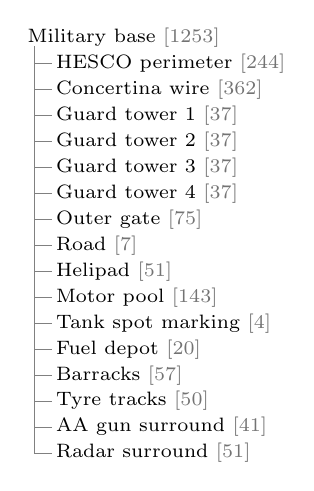
\begin{tikzpicture}[x=0.36cm,y=-0.33cm,font=\scriptsize]
\node[anchor=west,inner sep=0pt] (n0) at (0,0) {Military base \textcolor{black!55}{[1253]}};
\node[anchor=west,inner sep=0pt] (n1) at (1,1) {HESCO perimeter \textcolor{black!55}{[244]}};
\draw[black!50,thin] (0.25,0.35) |- (0.88,1);
\node[anchor=west,inner sep=0pt] (n2) at (1,2) {Concertina wire \textcolor{black!55}{[362]}};
\draw[black!50,thin] (0.25,0.35) |- (0.88,2);
\node[anchor=west,inner sep=0pt] (n3) at (1,3) {Guard tower 1 \textcolor{black!55}{[37]}};
\draw[black!50,thin] (0.25,0.35) |- (0.88,3);
\node[anchor=west,inner sep=0pt] (n4) at (1,4) {Guard tower 2 \textcolor{black!55}{[37]}};
\draw[black!50,thin] (0.25,0.35) |- (0.88,4);
\node[anchor=west,inner sep=0pt] (n5) at (1,5) {Guard tower 3 \textcolor{black!55}{[37]}};
\draw[black!50,thin] (0.25,0.35) |- (0.88,5);
\node[anchor=west,inner sep=0pt] (n6) at (1,6) {Guard tower 4 \textcolor{black!55}{[37]}};
\draw[black!50,thin] (0.25,0.35) |- (0.88,6);
\node[anchor=west,inner sep=0pt] (n7) at (1,7) {Outer gate \textcolor{black!55}{[75]}};
\draw[black!50,thin] (0.25,0.35) |- (0.88,7);
\node[anchor=west,inner sep=0pt] (n8) at (1,8) {Road \textcolor{black!55}{[7]}};
\draw[black!50,thin] (0.25,0.35) |- (0.88,8);
\node[anchor=west,inner sep=0pt] (n9) at (1,9) {Helipad \textcolor{black!55}{[51]}};
\draw[black!50,thin] (0.25,0.35) |- (0.88,9);
\node[anchor=west,inner sep=0pt] (n10) at (1,10) {Motor pool \textcolor{black!55}{[143]}};
\draw[black!50,thin] (0.25,0.35) |- (0.88,10);
\node[anchor=west,inner sep=0pt] (n11) at (1,11) {Tank spot marking \textcolor{black!55}{[4]}};
\draw[black!50,thin] (0.25,0.35) |- (0.88,11);
\node[anchor=west,inner sep=0pt] (n12) at (1,12) {Fuel depot \textcolor{black!55}{[20]}};
\draw[black!50,thin] (0.25,0.35) |- (0.88,12);
\node[anchor=west,inner sep=0pt] (n13) at (1,13) {Barracks \textcolor{black!55}{[57]}};
\draw[black!50,thin] (0.25,0.35) |- (0.88,13);
\node[anchor=west,inner sep=0pt] (n14) at (1,14) {Tyre tracks \textcolor{black!55}{[50]}};
\draw[black!50,thin] (0.25,0.35) |- (0.88,14);
\node[anchor=west,inner sep=0pt] (n15) at (1,15) {AA gun surround \textcolor{black!55}{[41]}};
\draw[black!50,thin] (0.25,0.35) |- (0.88,15);
\node[anchor=west,inner sep=0pt] (n16) at (1,16) {Radar surround \textcolor{black!55}{[51]}};
\draw[black!50,thin] (0.25,0.35) |- (0.88,16);
\end{tikzpicture}
\end{minipage}\hfill
\begin{minipage}[t]{0.40\linewidth}\vspace{0pt}
\captionsetup{type=figure}
\picfour{base_gate}{\linewidth}
\end{minipage}
\caption{Base hierarchy (left, from the export; the figure ``base\_gate'' (right) shows the outer gate with boom
barrier, booth and towers).}
\end{figure}

% ---------------------------------------------------------------------
\subsection{UAV with launcher rails}
\sheetfig{s03_uav}
The quadcopter (\partsUav{} parts, Phong) has a fuselage, canopy, four rotors, landing gear, LEDs, and the two-axis gimbal
\emph{body $\to$ gimbal yaw $\to$ gimbal pitch $\to$ \{lamp, lens, thermal camera, light frustum\}} shared by the thermal
tracker and the searchlight. Two \emph{launcher rails} (14 parts each) carry two missiles apiece (cylinder body, cone nose, four fins); a round is hidden on launch and
returns after the 10\,s reload (Section~\ref{sec:game}). Rotor-blur discs are translucent ($\alpha<1$, no shadow).

% ---------------------------------------------------------------------
\subsection{Intruder rover}
\sheetfig{s03_rover}
Each of the three intruders is a six-wheeled UGV with \partsRover{} parts: chassis, hull, motor box, six
cylinder wheels (axis turned onto $x$ by $R_y(90^\circ)$, spin $=R_z$), sphere hubs, five IR line sensors and a rotating
scanner. The motor box is the hottest part (thermal value 0.97), which the tracker locks on. The rovers share geometry with distinct part ids (\code{ROV-07}, \code{ROV2-07}, \code{ROV3-07}); a destroyed rover's parts become rigid debris (Section~\ref{sec:game}).

\begin{figure}[h]
\centering
\picsheet{sheet_construction_tank}{\linewidth}
\caption{\sheetcaption{sheet_construction_tank}}
\end{figure}
% ---------------------------------------------------------------------
\subsection{Main battle tank with 80 animated track links}
\sheetfig{s05_tank_chain}
\sheetfig{s03_tank_material}
The tank (\partsTank{} parts, Phong) parks at the motor pool facing the road. The hull carries plates, skirts and lights; the turret a cupola with a machine gun and smoke launchers; the gun is
\emph{gun pitch $\to$ barrel recoil $\to$ barrel, fume extractor, muzzle brake}. Each track has
$40$ link cubes ($\nTrackLinks$ in total) plus seven road wheels, sprocket, idler and rollers. Link
transforms are set each frame from the arc length along a closed stadium-shaped
path (Section~\ref{sec:control}); T80 checks that all 80 links stay on the path (max distance $0$\,m).

\begin{figure}[h]
\centering
\begin{minipage}[t]{0.31\linewidth}\vspace{0pt}% generated by report/gen_tables.py from build/scene_export.json -- do not edit
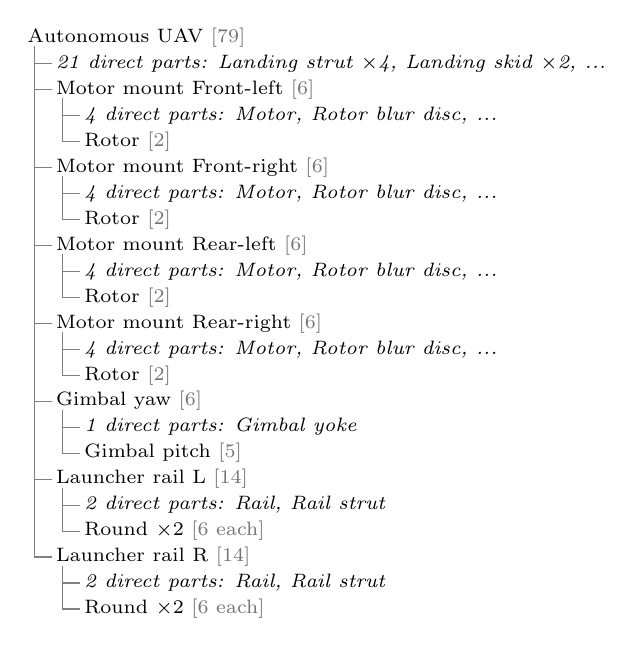
\begin{tikzpicture}[x=0.36cm,y=-0.33cm,font=\scriptsize]
\node[anchor=west,inner sep=0pt] (n0) at (0,0) {Autonomous UAV \textcolor{black!55}{[79]}};
\node[anchor=west,inner sep=0pt] (n1) at (1,1) {\textit{21 direct parts: Landing strut $\times$4, Landing skid $\times$2, ...}};
\draw[black!50,thin] (0.25,0.35) |- (0.88,1);
\node[anchor=west,inner sep=0pt] (n2) at (1,2) {Motor mount Front-left \textcolor{black!55}{[6]}};
\draw[black!50,thin] (0.25,0.35) |- (0.88,2);
\node[anchor=west,inner sep=0pt] (n3) at (2,3) {\textit{4 direct parts: Motor, Rotor blur disc, ...}};
\draw[black!50,thin] (1.25,2.35) |- (1.88,3);
\node[anchor=west,inner sep=0pt] (n4) at (2,4) {Rotor \textcolor{black!55}{[2]}};
\draw[black!50,thin] (1.25,2.35) |- (1.88,4);
\node[anchor=west,inner sep=0pt] (n5) at (1,5) {Motor mount Front-right \textcolor{black!55}{[6]}};
\draw[black!50,thin] (0.25,0.35) |- (0.88,5);
\node[anchor=west,inner sep=0pt] (n6) at (2,6) {\textit{4 direct parts: Motor, Rotor blur disc, ...}};
\draw[black!50,thin] (1.25,5.35) |- (1.88,6);
\node[anchor=west,inner sep=0pt] (n7) at (2,7) {Rotor \textcolor{black!55}{[2]}};
\draw[black!50,thin] (1.25,5.35) |- (1.88,7);
\node[anchor=west,inner sep=0pt] (n8) at (1,8) {Motor mount Rear-left \textcolor{black!55}{[6]}};
\draw[black!50,thin] (0.25,0.35) |- (0.88,8);
\node[anchor=west,inner sep=0pt] (n9) at (2,9) {\textit{4 direct parts: Motor, Rotor blur disc, ...}};
\draw[black!50,thin] (1.25,8.35) |- (1.88,9);
\node[anchor=west,inner sep=0pt] (n10) at (2,10) {Rotor \textcolor{black!55}{[2]}};
\draw[black!50,thin] (1.25,8.35) |- (1.88,10);
\node[anchor=west,inner sep=0pt] (n11) at (1,11) {Motor mount Rear-right \textcolor{black!55}{[6]}};
\draw[black!50,thin] (0.25,0.35) |- (0.88,11);
\node[anchor=west,inner sep=0pt] (n12) at (2,12) {\textit{4 direct parts: Motor, Rotor blur disc, ...}};
\draw[black!50,thin] (1.25,11.35) |- (1.88,12);
\node[anchor=west,inner sep=0pt] (n13) at (2,13) {Rotor \textcolor{black!55}{[2]}};
\draw[black!50,thin] (1.25,11.35) |- (1.88,13);
\node[anchor=west,inner sep=0pt] (n14) at (1,14) {Gimbal yaw \textcolor{black!55}{[6]}};
\draw[black!50,thin] (0.25,0.35) |- (0.88,14);
\node[anchor=west,inner sep=0pt] (n15) at (2,15) {\textit{1 direct parts: Gimbal yoke}};
\draw[black!50,thin] (1.25,14.35) |- (1.88,15);
\node[anchor=west,inner sep=0pt] (n16) at (2,16) {Gimbal pitch \textcolor{black!55}{[5]}};
\draw[black!50,thin] (1.25,14.35) |- (1.88,16);
\node[anchor=west,inner sep=0pt] (n17) at (1,17) {Launcher rail L \textcolor{black!55}{[14]}};
\draw[black!50,thin] (0.25,0.35) |- (0.88,17);
\node[anchor=west,inner sep=0pt] (n18) at (2,18) {\textit{2 direct parts: Rail, Rail strut}};
\draw[black!50,thin] (1.25,17.35) |- (1.88,18);
\node[anchor=west,inner sep=0pt] (n19) at (2,19) {Round $\times$2 \textcolor{black!55}{[6 each]}};
\draw[black!50,thin] (1.25,17.35) |- (1.88,19);
\node[anchor=west,inner sep=0pt] (n20) at (1,20) {Launcher rail R \textcolor{black!55}{[14]}};
\draw[black!50,thin] (0.25,0.35) |- (0.88,20);
\node[anchor=west,inner sep=0pt] (n21) at (2,21) {\textit{2 direct parts: Rail, Rail strut}};
\draw[black!50,thin] (1.25,20.35) |- (1.88,21);
\node[anchor=west,inner sep=0pt] (n22) at (2,22) {Round $\times$2 \textcolor{black!55}{[6 each]}};
\draw[black!50,thin] (1.25,20.35) |- (1.88,22);
\end{tikzpicture}
\end{minipage}\hfill
\begin{minipage}[t]{0.31\linewidth}\vspace{0pt}% generated by report/gen_tables.py from build/scene_export.json -- do not edit
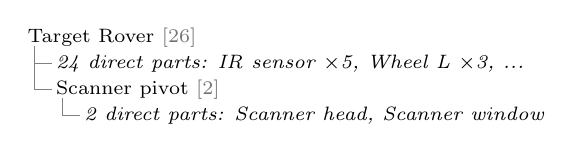
\begin{tikzpicture}[x=0.36cm,y=-0.33cm,font=\scriptsize]
\node[anchor=west,inner sep=0pt] (n0) at (0,0) {Target Rover \textcolor{black!55}{[26]}};
\node[anchor=west,inner sep=0pt] (n1) at (1,1) {\textit{24 direct parts: IR sensor $\times$5, Wheel L $\times$3, ...}};
\draw[black!50,thin] (0.25,0.35) |- (0.88,1);
\node[anchor=west,inner sep=0pt] (n2) at (1,2) {Scanner pivot \textcolor{black!55}{[2]}};
\draw[black!50,thin] (0.25,0.35) |- (0.88,2);
\node[anchor=west,inner sep=0pt] (n3) at (2,3) {\textit{2 direct parts: Scanner head, Scanner window}};
\draw[black!50,thin] (1.25,2.35) |- (1.88,3);
\end{tikzpicture}
\end{minipage}\hfill
\begin{minipage}[t]{0.35\linewidth}\vspace{0pt}% generated by report/gen_tables.py from build/scene_export.json -- do not edit
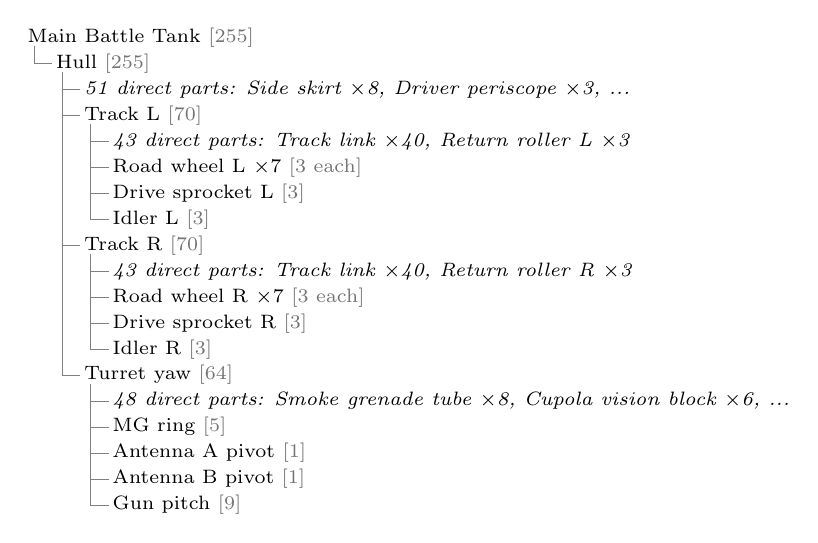
\begin{tikzpicture}[x=0.36cm,y=-0.33cm,font=\scriptsize]
\node[anchor=west,inner sep=0pt] (n0) at (0,0) {Main Battle Tank \textcolor{black!55}{[255]}};
\node[anchor=west,inner sep=0pt] (n1) at (1,1) {Hull \textcolor{black!55}{[255]}};
\draw[black!50,thin] (0.25,0.35) |- (0.88,1);
\node[anchor=west,inner sep=0pt] (n2) at (2,2) {\textit{51 direct parts: Side skirt $\times$8, Driver periscope $\times$3, ...}};
\draw[black!50,thin] (1.25,1.35) |- (1.88,2);
\node[anchor=west,inner sep=0pt] (n3) at (2,3) {Track L \textcolor{black!55}{[70]}};
\draw[black!50,thin] (1.25,1.35) |- (1.88,3);
\node[anchor=west,inner sep=0pt] (n4) at (3,4) {\textit{43 direct parts: Track link $\times$40, Return roller L $\times$3}};
\draw[black!50,thin] (2.25,3.35) |- (2.88,4);
\node[anchor=west,inner sep=0pt] (n5) at (3,5) {Road wheel L $\times$7 \textcolor{black!55}{[3 each]}};
\draw[black!50,thin] (2.25,3.35) |- (2.88,5);
\node[anchor=west,inner sep=0pt] (n6) at (3,6) {Drive sprocket L \textcolor{black!55}{[3]}};
\draw[black!50,thin] (2.25,3.35) |- (2.88,6);
\node[anchor=west,inner sep=0pt] (n7) at (3,7) {Idler L \textcolor{black!55}{[3]}};
\draw[black!50,thin] (2.25,3.35) |- (2.88,7);
\node[anchor=west,inner sep=0pt] (n8) at (2,8) {Track R \textcolor{black!55}{[70]}};
\draw[black!50,thin] (1.25,1.35) |- (1.88,8);
\node[anchor=west,inner sep=0pt] (n9) at (3,9) {\textit{43 direct parts: Track link $\times$40, Return roller R $\times$3}};
\draw[black!50,thin] (2.25,8.35) |- (2.88,9);
\node[anchor=west,inner sep=0pt] (n10) at (3,10) {Road wheel R $\times$7 \textcolor{black!55}{[3 each]}};
\draw[black!50,thin] (2.25,8.35) |- (2.88,10);
\node[anchor=west,inner sep=0pt] (n11) at (3,11) {Drive sprocket R \textcolor{black!55}{[3]}};
\draw[black!50,thin] (2.25,8.35) |- (2.88,11);
\node[anchor=west,inner sep=0pt] (n12) at (3,12) {Idler R \textcolor{black!55}{[3]}};
\draw[black!50,thin] (2.25,8.35) |- (2.88,12);
\node[anchor=west,inner sep=0pt] (n13) at (2,13) {Turret yaw \textcolor{black!55}{[64]}};
\draw[black!50,thin] (1.25,1.35) |- (1.88,13);
\node[anchor=west,inner sep=0pt] (n14) at (3,14) {\textit{48 direct parts: Smoke grenade tube $\times$8, Cupola vision block $\times$6, ...}};
\draw[black!50,thin] (2.25,13.35) |- (2.88,14);
\node[anchor=west,inner sep=0pt] (n15) at (3,15) {MG ring \textcolor{black!55}{[5]}};
\draw[black!50,thin] (2.25,13.35) |- (2.88,15);
\node[anchor=west,inner sep=0pt] (n16) at (3,16) {Antenna A pivot \textcolor{black!55}{[1]}};
\draw[black!50,thin] (2.25,13.35) |- (2.88,16);
\node[anchor=west,inner sep=0pt] (n17) at (3,17) {Antenna B pivot \textcolor{black!55}{[1]}};
\draw[black!50,thin] (2.25,13.35) |- (2.88,17);
\node[anchor=west,inner sep=0pt] (n18) at (3,18) {Gun pitch \textcolor{black!55}{[9]}};
\draw[black!50,thin] (2.25,13.35) |- (2.88,18);
\end{tikzpicture}
\end{minipage}
\caption{Hierarchies of the UAV, the first rover and the tank (export). In the tank, \emph{Hull} owns the suspension heave and the pitch spring, \emph{Turret yaw} is
stabilised against the hull, and both tracks hang under the hull.}
\label{fig:tree-ground}
\end{figure}

% ---------------------------------------------------------------------
\subsection{AA Gatling gun with the six-barrel cluster}
\sheetfig{s03_aagun}
The anti-aircraft gun (\partsAa{} parts, Phong) stands at $(21,-19)$: \emph{mount yaw (360$^\circ$) $\to$ cradle pitch ($-5\ldots85^\circ$) $\to$ barrel cluster}. The cluster is six
2\,m cylinders every $60^\circ$ on a $0.14$\,m circle, spinning about its axis; a pool of 20 shell casings is ejected while firing. The mount also carries a
radome with a rotating search antenna.

% ---------------------------------------------------------------------
\subsection{Helicopter with a cyclic rotor head}
\sheetfig{s03_helicopter}
The scout helicopter (\partsHeli{} parts, MH-6 class) sits on the helipad at $(20.3,\,17)$:
\emph{root (position, yaw) $\to$ body (pitch, roll) $\to$ \{cabin, boom, skids, rotor head $\to$ tip-path plane $\to$
spinning rotor $\to$ five pivots $\to$ flap nodes $\to$ blades; tail rotor; searchlight pan $\to$ tilt\}}, depth 7 at the deepest leaf. Each blade is a $0.22\times0.03\times3.9$\,m cube centred 1.95\,m from the hinge,
so a flap rotation turns it about its root. T96 counts 68 leaves.

% ---------------------------------------------------------------------
\subsection{Radar}
\sheetfig{s03_radar}
The radar (\partsRadar{} parts) at $(29,-3)$ has a plinth, lattice mast, shelter and an
\emph{azimuth head $\to$ elevation yoke $\to$ antenna array} hierarchy. The array is $7\times3$ cube tiles
$0.64\times0.78\times0.05$\,m on a 5\,m arc in $7.5^\circ$ steps (T99), with a feed horn, an IFF bar and a red beacon blinking at 1\,Hz.

\begin{figure}[h]
\centering
\begin{minipage}[t]{0.55\linewidth}\vspace{0pt}% generated by report/gen_tables.py from build/scene_export.json -- do not edit
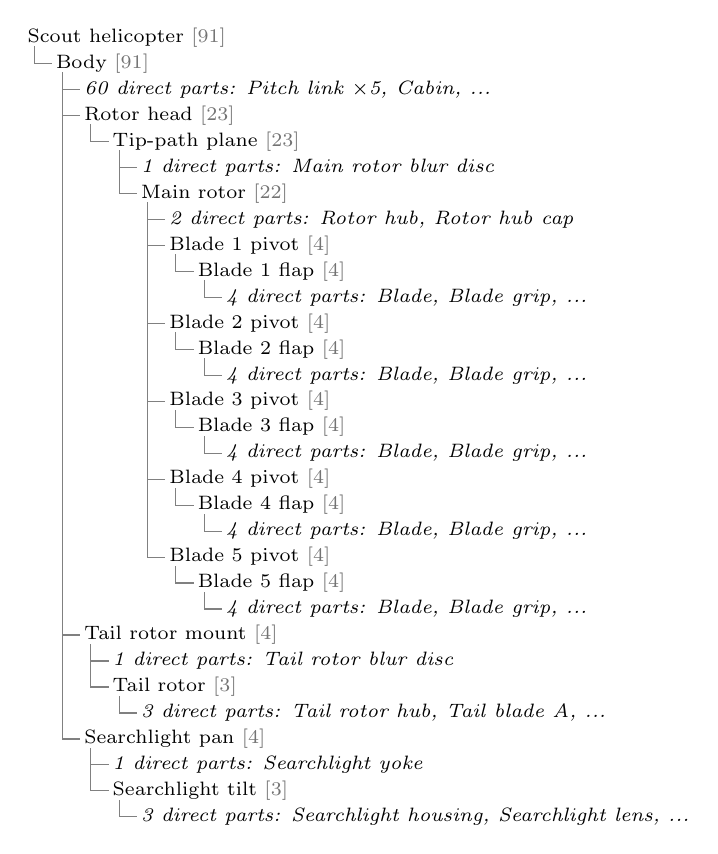
\begin{tikzpicture}[x=0.36cm,y=-0.33cm,font=\scriptsize]
\node[anchor=west,inner sep=0pt] (n0) at (0,0) {Scout helicopter \textcolor{black!55}{[91]}};
\node[anchor=west,inner sep=0pt] (n1) at (1,1) {Body \textcolor{black!55}{[91]}};
\draw[black!50,thin] (0.25,0.35) |- (0.88,1);
\node[anchor=west,inner sep=0pt] (n2) at (2,2) {\textit{60 direct parts: Pitch link $\times$5, Cabin, ...}};
\draw[black!50,thin] (1.25,1.35) |- (1.88,2);
\node[anchor=west,inner sep=0pt] (n3) at (2,3) {Rotor head \textcolor{black!55}{[23]}};
\draw[black!50,thin] (1.25,1.35) |- (1.88,3);
\node[anchor=west,inner sep=0pt] (n4) at (3,4) {Tip-path plane \textcolor{black!55}{[23]}};
\draw[black!50,thin] (2.25,3.35) |- (2.88,4);
\node[anchor=west,inner sep=0pt] (n5) at (4,5) {\textit{1 direct parts: Main rotor blur disc}};
\draw[black!50,thin] (3.25,4.35) |- (3.88,5);
\node[anchor=west,inner sep=0pt] (n6) at (4,6) {Main rotor \textcolor{black!55}{[22]}};
\draw[black!50,thin] (3.25,4.35) |- (3.88,6);
\node[anchor=west,inner sep=0pt] (n7) at (5,7) {\textit{2 direct parts: Rotor hub, Rotor hub cap}};
\draw[black!50,thin] (4.25,6.35) |- (4.88,7);
\node[anchor=west,inner sep=0pt] (n8) at (5,8) {Blade 1 pivot \textcolor{black!55}{[4]}};
\draw[black!50,thin] (4.25,6.35) |- (4.88,8);
\node[anchor=west,inner sep=0pt] (n9) at (6,9) {Blade 1 flap \textcolor{black!55}{[4]}};
\draw[black!50,thin] (5.25,8.35) |- (5.88,9);
\node[anchor=west,inner sep=0pt] (n10) at (7,10) {\textit{4 direct parts: Blade, Blade grip, ...}};
\draw[black!50,thin] (6.25,9.35) |- (6.88,10);
\node[anchor=west,inner sep=0pt] (n11) at (5,11) {Blade 2 pivot \textcolor{black!55}{[4]}};
\draw[black!50,thin] (4.25,6.35) |- (4.88,11);
\node[anchor=west,inner sep=0pt] (n12) at (6,12) {Blade 2 flap \textcolor{black!55}{[4]}};
\draw[black!50,thin] (5.25,11.35) |- (5.88,12);
\node[anchor=west,inner sep=0pt] (n13) at (7,13) {\textit{4 direct parts: Blade, Blade grip, ...}};
\draw[black!50,thin] (6.25,12.35) |- (6.88,13);
\node[anchor=west,inner sep=0pt] (n14) at (5,14) {Blade 3 pivot \textcolor{black!55}{[4]}};
\draw[black!50,thin] (4.25,6.35) |- (4.88,14);
\node[anchor=west,inner sep=0pt] (n15) at (6,15) {Blade 3 flap \textcolor{black!55}{[4]}};
\draw[black!50,thin] (5.25,14.35) |- (5.88,15);
\node[anchor=west,inner sep=0pt] (n16) at (7,16) {\textit{4 direct parts: Blade, Blade grip, ...}};
\draw[black!50,thin] (6.25,15.35) |- (6.88,16);
\node[anchor=west,inner sep=0pt] (n17) at (5,17) {Blade 4 pivot \textcolor{black!55}{[4]}};
\draw[black!50,thin] (4.25,6.35) |- (4.88,17);
\node[anchor=west,inner sep=0pt] (n18) at (6,18) {Blade 4 flap \textcolor{black!55}{[4]}};
\draw[black!50,thin] (5.25,17.35) |- (5.88,18);
\node[anchor=west,inner sep=0pt] (n19) at (7,19) {\textit{4 direct parts: Blade, Blade grip, ...}};
\draw[black!50,thin] (6.25,18.35) |- (6.88,19);
\node[anchor=west,inner sep=0pt] (n20) at (5,20) {Blade 5 pivot \textcolor{black!55}{[4]}};
\draw[black!50,thin] (4.25,6.35) |- (4.88,20);
\node[anchor=west,inner sep=0pt] (n21) at (6,21) {Blade 5 flap \textcolor{black!55}{[4]}};
\draw[black!50,thin] (5.25,20.35) |- (5.88,21);
\node[anchor=west,inner sep=0pt] (n22) at (7,22) {\textit{4 direct parts: Blade, Blade grip, ...}};
\draw[black!50,thin] (6.25,21.35) |- (6.88,22);
\node[anchor=west,inner sep=0pt] (n23) at (2,23) {Tail rotor mount \textcolor{black!55}{[4]}};
\draw[black!50,thin] (1.25,1.35) |- (1.88,23);
\node[anchor=west,inner sep=0pt] (n24) at (3,24) {\textit{1 direct parts: Tail rotor blur disc}};
\draw[black!50,thin] (2.25,23.35) |- (2.88,24);
\node[anchor=west,inner sep=0pt] (n25) at (3,25) {Tail rotor \textcolor{black!55}{[3]}};
\draw[black!50,thin] (2.25,23.35) |- (2.88,25);
\node[anchor=west,inner sep=0pt] (n26) at (4,26) {\textit{3 direct parts: Tail rotor hub, Tail blade A, ...}};
\draw[black!50,thin] (3.25,25.35) |- (3.88,26);
\node[anchor=west,inner sep=0pt] (n27) at (2,27) {Searchlight pan \textcolor{black!55}{[4]}};
\draw[black!50,thin] (1.25,1.35) |- (1.88,27);
\node[anchor=west,inner sep=0pt] (n28) at (3,28) {\textit{1 direct parts: Searchlight yoke}};
\draw[black!50,thin] (2.25,27.35) |- (2.88,28);
\node[anchor=west,inner sep=0pt] (n29) at (3,29) {Searchlight tilt \textcolor{black!55}{[3]}};
\draw[black!50,thin] (2.25,27.35) |- (2.88,29);
\node[anchor=west,inner sep=0pt] (n30) at (4,30) {\textit{3 direct parts: Searchlight housing, Searchlight lens, ...}};
\draw[black!50,thin] (3.25,29.35) |- (3.88,30);
\end{tikzpicture}
\end{minipage}\hfill
\begin{minipage}[t]{0.42\linewidth}\vspace{0pt}% generated by report/gen_tables.py from build/scene_export.json -- do not edit
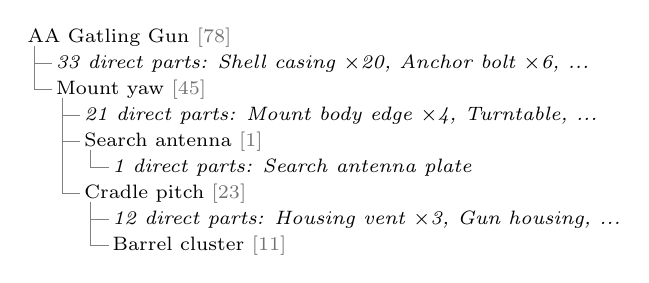
\begin{tikzpicture}[x=0.36cm,y=-0.33cm,font=\scriptsize]
\node[anchor=west,inner sep=0pt] (n0) at (0,0) {AA Gatling Gun \textcolor{black!55}{[78]}};
\node[anchor=west,inner sep=0pt] (n1) at (1,1) {\textit{33 direct parts: Shell casing $\times$20, Anchor bolt $\times$6, ...}};
\draw[black!50,thin] (0.25,0.35) |- (0.88,1);
\node[anchor=west,inner sep=0pt] (n2) at (1,2) {Mount yaw \textcolor{black!55}{[45]}};
\draw[black!50,thin] (0.25,0.35) |- (0.88,2);
\node[anchor=west,inner sep=0pt] (n3) at (2,3) {\textit{21 direct parts: Mount body edge $\times$4, Turntable, ...}};
\draw[black!50,thin] (1.25,2.35) |- (1.88,3);
\node[anchor=west,inner sep=0pt] (n4) at (2,4) {Search antenna \textcolor{black!55}{[1]}};
\draw[black!50,thin] (1.25,2.35) |- (1.88,4);
\node[anchor=west,inner sep=0pt] (n5) at (3,5) {\textit{1 direct parts: Search antenna plate}};
\draw[black!50,thin] (2.25,4.35) |- (2.88,5);
\node[anchor=west,inner sep=0pt] (n6) at (2,6) {Cradle pitch \textcolor{black!55}{[23]}};
\draw[black!50,thin] (1.25,2.35) |- (1.88,6);
\node[anchor=west,inner sep=0pt] (n7) at (3,7) {\textit{12 direct parts: Housing vent $\times$3, Gun housing, ...}};
\draw[black!50,thin] (2.25,6.35) |- (2.88,7);
\node[anchor=west,inner sep=0pt] (n8) at (3,8) {Barrel cluster \textcolor{black!55}{[11]}};
\draw[black!50,thin] (2.25,6.35) |- (2.88,8);
\end{tikzpicture}
\\[3mm]% generated by report/gen_tables.py from build/scene_export.json -- do not edit
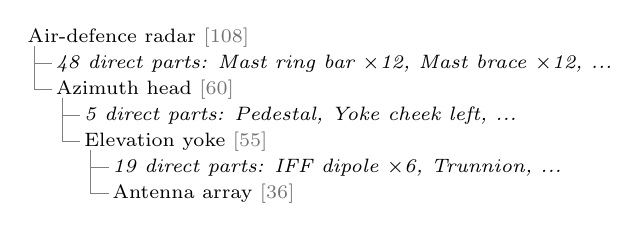
\begin{tikzpicture}[x=0.36cm,y=-0.33cm,font=\scriptsize]
\node[anchor=west,inner sep=0pt] (n0) at (0,0) {Air-defence radar \textcolor{black!55}{[108]}};
\node[anchor=west,inner sep=0pt] (n1) at (1,1) {\textit{48 direct parts: Mast ring bar $\times$12, Mast brace $\times$12, ...}};
\draw[black!50,thin] (0.25,0.35) |- (0.88,1);
\node[anchor=west,inner sep=0pt] (n2) at (1,2) {Azimuth head \textcolor{black!55}{[60]}};
\draw[black!50,thin] (0.25,0.35) |- (0.88,2);
\node[anchor=west,inner sep=0pt] (n3) at (2,3) {\textit{5 direct parts: Pedestal, Yoke cheek left, ...}};
\draw[black!50,thin] (1.25,2.35) |- (1.88,3);
\node[anchor=west,inner sep=0pt] (n4) at (2,4) {Elevation yoke \textcolor{black!55}{[55]}};
\draw[black!50,thin] (1.25,2.35) |- (1.88,4);
\node[anchor=west,inner sep=0pt] (n5) at (3,5) {\textit{19 direct parts: IFF dipole $\times$6, Trunnion, ...}};
\draw[black!50,thin] (2.25,4.35) |- (2.88,5);
\node[anchor=west,inner sep=0pt] (n6) at (3,6) {Antenna array \textcolor{black!55}{[36]}};
\draw[black!50,thin] (2.25,4.35) |- (2.88,6);
\end{tikzpicture}
\end{minipage}
\caption{Hierarchies of the helicopter (left; the tip-path-plane node tilts with the cyclic and each blade flaps and feathers under its own \emph{Blade $i$ flap} node), the AA gun and
the radar (right), from the export. Captures of the same machines are in Fig.~\ref{fig:machines}.}
\label{fig:tree-air}
\end{figure}

% ---------------------------------------------------------------------
\subsection{Gate barrier, windsock and flag}
\sheetfig{s03_gate}
\sheetfig{s03_flag}
Three animated base objects: the possessable \emph{boom barrier} (\partsBarrier{} parts, five red and five white stripes, counterweight, lamps), the \emph{windsock} (\partsWindsock{} parts: pole, swivel, five chained
segments) and the \emph{flag} (\partsFlag{} parts: a flag of 12 chained strips). Windsock and flag share one wind function.

\begin{figure}[h]
\centering
\begin{minipage}[t]{0.32\linewidth}\vspace{0pt}% generated by report/gen_tables.py from build/scene_export.json -- do not edit
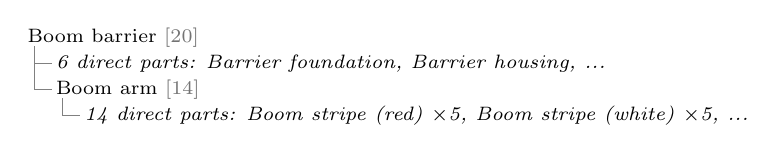
\begin{tikzpicture}[x=0.36cm,y=-0.33cm,font=\scriptsize]
\node[anchor=west,inner sep=0pt] (n0) at (0,0) {Boom barrier \textcolor{black!55}{[20]}};
\node[anchor=west,inner sep=0pt] (n1) at (1,1) {\textit{6 direct parts: Barrier foundation, Barrier housing, ...}};
\draw[black!50,thin] (0.25,0.35) |- (0.88,1);
\node[anchor=west,inner sep=0pt] (n2) at (1,2) {Boom arm \textcolor{black!55}{[14]}};
\draw[black!50,thin] (0.25,0.35) |- (0.88,2);
\node[anchor=west,inner sep=0pt] (n3) at (2,3) {\textit{14 direct parts: Boom stripe (red) $\times$5, Boom stripe (white) $\times$5, ...}};
\draw[black!50,thin] (1.25,2.35) |- (1.88,3);
\end{tikzpicture}
\end{minipage}\hfill
\begin{minipage}[t]{0.32\linewidth}\vspace{0pt}% generated by report/gen_tables.py from build/scene_export.json -- do not edit
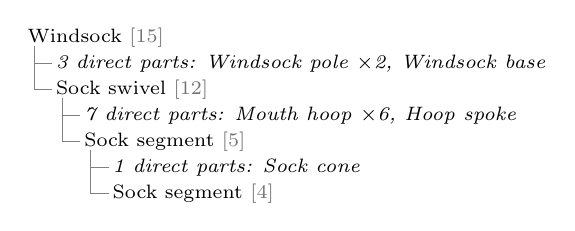
\begin{tikzpicture}[x=0.36cm,y=-0.33cm,font=\scriptsize]
\node[anchor=west,inner sep=0pt] (n0) at (0,0) {Windsock \textcolor{black!55}{[15]}};
\node[anchor=west,inner sep=0pt] (n1) at (1,1) {\textit{3 direct parts: Windsock pole $\times$2, Windsock base}};
\draw[black!50,thin] (0.25,0.35) |- (0.88,1);
\node[anchor=west,inner sep=0pt] (n2) at (1,2) {Sock swivel \textcolor{black!55}{[12]}};
\draw[black!50,thin] (0.25,0.35) |- (0.88,2);
\node[anchor=west,inner sep=0pt] (n3) at (2,3) {\textit{7 direct parts: Mouth hoop $\times$6, Hoop spoke}};
\draw[black!50,thin] (1.25,2.35) |- (1.88,3);
\node[anchor=west,inner sep=0pt] (n4) at (2,4) {Sock segment \textcolor{black!55}{[5]}};
\draw[black!50,thin] (1.25,2.35) |- (1.88,4);
\node[anchor=west,inner sep=0pt] (n5) at (3,5) {\textit{1 direct parts: Sock cone}};
\draw[black!50,thin] (2.25,4.35) |- (2.88,5);
\node[anchor=west,inner sep=0pt] (n6) at (3,6) {Sock segment \textcolor{black!55}{[4]}};
\draw[black!50,thin] (2.25,4.35) |- (2.88,6);
\end{tikzpicture}
\end{minipage}\hfill
\begin{minipage}[t]{0.32\linewidth}\vspace{0pt}% generated by report/gen_tables.py from build/scene_export.json -- do not edit
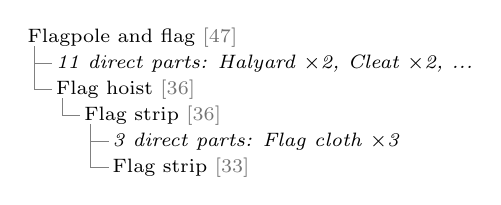
\begin{tikzpicture}[x=0.36cm,y=-0.33cm,font=\scriptsize]
\node[anchor=west,inner sep=0pt] (n0) at (0,0) {Flagpole and flag \textcolor{black!55}{[47]}};
\node[anchor=west,inner sep=0pt] (n1) at (1,1) {\textit{11 direct parts: Halyard $\times$2, Cleat $\times$2, ...}};
\draw[black!50,thin] (0.25,0.35) |- (0.88,1);
\node[anchor=west,inner sep=0pt] (n2) at (1,2) {Flag hoist \textcolor{black!55}{[36]}};
\draw[black!50,thin] (0.25,0.35) |- (0.88,2);
\node[anchor=west,inner sep=0pt] (n3) at (2,3) {Flag strip \textcolor{black!55}{[36]}};
\draw[black!50,thin] (1.25,2.35) |- (1.88,3);
\node[anchor=west,inner sep=0pt] (n4) at (3,4) {\textit{3 direct parts: Flag cloth $\times$3}};
\draw[black!50,thin] (2.25,3.35) |- (2.88,4);
\node[anchor=west,inner sep=0pt] (n5) at (3,5) {Flag strip \textcolor{black!55}{[33]}};
\draw[black!50,thin] (2.25,3.35) |- (2.88,5);
\end{tikzpicture}
\end{minipage}
\caption{Hierarchies of the boom barrier, the windsock and the flag (export). The windsock and the flag are chains in
which every segment is the child of the previous one.}
\end{figure}

% ---------------------------------------------------------------------
\subsection{Environment, terrain and backdrop}
The Gouraud environment (\partsEnv{} parts) holds the compound's fence, watchtower, sandbag walls, tent, supply caches, radio mast,
spruces of cone whorls, broadleaf trees of sphere clumps, bushes, boulders and military dressing (HESCO blocks, jersey chicane, fighting position). The trench strip and the bunker
footprint are cleared of vegetation (T78). The terrain (130 rings $\times$ 384 slices, 49\,921
vertices, 97\,440 triangles, trench hole; T13/T61) has a levelled bunker pad,
a creek, a track, a berm and a mound over the bunker roof (T60). The backdrop (\partsBackdrop{} parts:
hills, a 46-pine tree line, a far radio tower at 100\,m) starts beyond the mesh (T79: nearest part 38.0\,m).

\begin{figure}[h]
\centering
\begin{minipage}[t]{0.6\linewidth}\vspace{0pt}% generated by report/gen_tables.py from build/scene_export.json -- do not edit
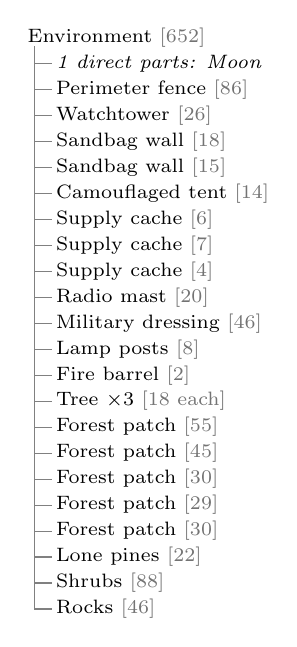
\begin{tikzpicture}[x=0.36cm,y=-0.33cm,font=\scriptsize]
\node[anchor=west,inner sep=0pt] (n0) at (0,0) {Environment \textcolor{black!55}{[652]}};
\node[anchor=west,inner sep=0pt] (n1) at (1,1) {\textit{1 direct parts: Moon}};
\draw[black!50,thin] (0.25,0.35) |- (0.88,1);
\node[anchor=west,inner sep=0pt] (n2) at (1,2) {Perimeter fence \textcolor{black!55}{[86]}};
\draw[black!50,thin] (0.25,0.35) |- (0.88,2);
\node[anchor=west,inner sep=0pt] (n3) at (1,3) {Watchtower \textcolor{black!55}{[26]}};
\draw[black!50,thin] (0.25,0.35) |- (0.88,3);
\node[anchor=west,inner sep=0pt] (n4) at (1,4) {Sandbag wall \textcolor{black!55}{[18]}};
\draw[black!50,thin] (0.25,0.35) |- (0.88,4);
\node[anchor=west,inner sep=0pt] (n5) at (1,5) {Sandbag wall \textcolor{black!55}{[15]}};
\draw[black!50,thin] (0.25,0.35) |- (0.88,5);
\node[anchor=west,inner sep=0pt] (n6) at (1,6) {Camouflaged tent \textcolor{black!55}{[14]}};
\draw[black!50,thin] (0.25,0.35) |- (0.88,6);
\node[anchor=west,inner sep=0pt] (n7) at (1,7) {Supply cache \textcolor{black!55}{[6]}};
\draw[black!50,thin] (0.25,0.35) |- (0.88,7);
\node[anchor=west,inner sep=0pt] (n8) at (1,8) {Supply cache \textcolor{black!55}{[7]}};
\draw[black!50,thin] (0.25,0.35) |- (0.88,8);
\node[anchor=west,inner sep=0pt] (n9) at (1,9) {Supply cache \textcolor{black!55}{[4]}};
\draw[black!50,thin] (0.25,0.35) |- (0.88,9);
\node[anchor=west,inner sep=0pt] (n10) at (1,10) {Radio mast \textcolor{black!55}{[20]}};
\draw[black!50,thin] (0.25,0.35) |- (0.88,10);
\node[anchor=west,inner sep=0pt] (n11) at (1,11) {Military dressing \textcolor{black!55}{[46]}};
\draw[black!50,thin] (0.25,0.35) |- (0.88,11);
\node[anchor=west,inner sep=0pt] (n12) at (1,12) {Lamp posts \textcolor{black!55}{[8]}};
\draw[black!50,thin] (0.25,0.35) |- (0.88,12);
\node[anchor=west,inner sep=0pt] (n13) at (1,13) {Fire barrel \textcolor{black!55}{[2]}};
\draw[black!50,thin] (0.25,0.35) |- (0.88,13);
\node[anchor=west,inner sep=0pt] (n14) at (1,14) {Tree $\times$3 \textcolor{black!55}{[18 each]}};
\draw[black!50,thin] (0.25,0.35) |- (0.88,14);
\node[anchor=west,inner sep=0pt] (n15) at (1,15) {Forest patch \textcolor{black!55}{[55]}};
\draw[black!50,thin] (0.25,0.35) |- (0.88,15);
\node[anchor=west,inner sep=0pt] (n16) at (1,16) {Forest patch \textcolor{black!55}{[45]}};
\draw[black!50,thin] (0.25,0.35) |- (0.88,16);
\node[anchor=west,inner sep=0pt] (n17) at (1,17) {Forest patch \textcolor{black!55}{[30]}};
\draw[black!50,thin] (0.25,0.35) |- (0.88,17);
\node[anchor=west,inner sep=0pt] (n18) at (1,18) {Forest patch \textcolor{black!55}{[29]}};
\draw[black!50,thin] (0.25,0.35) |- (0.88,18);
\node[anchor=west,inner sep=0pt] (n19) at (1,19) {Forest patch \textcolor{black!55}{[30]}};
\draw[black!50,thin] (0.25,0.35) |- (0.88,19);
\node[anchor=west,inner sep=0pt] (n20) at (1,20) {Lone pines \textcolor{black!55}{[22]}};
\draw[black!50,thin] (0.25,0.35) |- (0.88,20);
\node[anchor=west,inner sep=0pt] (n21) at (1,21) {Shrubs \textcolor{black!55}{[88]}};
\draw[black!50,thin] (0.25,0.35) |- (0.88,21);
\node[anchor=west,inner sep=0pt] (n22) at (1,22) {Rocks \textcolor{black!55}{[46]}};
\draw[black!50,thin] (0.25,0.35) |- (0.88,22);
\end{tikzpicture}
\end{minipage}\hfill
\begin{minipage}[t]{0.36\linewidth}\vspace{0pt}\footnotesize
\begin{tabular}{@{}ll@{}}\toprule
Terrain mesh & 130 $\times$ 384, $r=36$\,m\\
Creek depth & $-0.41$\,m (T42)\\
Berm & $+0.44$\,m (T42)\\
Apron level & $-0.30$\,m\\
Far ground top & $-0.35$\,m (T43)\\\bottomrule
\end{tabular}
\end{minipage}
\caption{Environment groups (export, depth 1) and terrain values measured by T42/T43.}
\end{figure}
